\documentclass[border=4pt]{standalone}
\usepackage{fontspec}
\usepackage{amsmath}
\usepackage{unicode-math}
\setmainfont{Latin Modern Roman}
\setmathfont{Latin Modern Math}
\usepackage{pgfplots}
\usepackage{pgfplotstable}
\pgfplotsset{compat=1.18}
\usepackage{tkz-euclide}
\usetikzlibrary{arrows.meta,calc,angles,quotes,patterns,3d,backgrounds}
\definecolor{ink}{HTML}{123428}
\definecolor{asy}{HTML}{475569}
\definecolor{mint}{HTML}{86e0bd}
\tikzset{asym/.style={asy, line width=0.9pt, dash pattern=on 5pt off 3.5pt},
         guide/.style={gray!70, line width=0.6pt, densely dotted},
         dot/.style={circle, inner sep=0pt, minimum size=5pt, draw=white, line width=0.5pt},
         odot/.style={circle, inner sep=0pt, minimum size=5.5pt, fill=white, line width=1pt},
         lab/.style={font=\footnotesize, inner sep=1.5pt, text=ink}}
\begin{document}
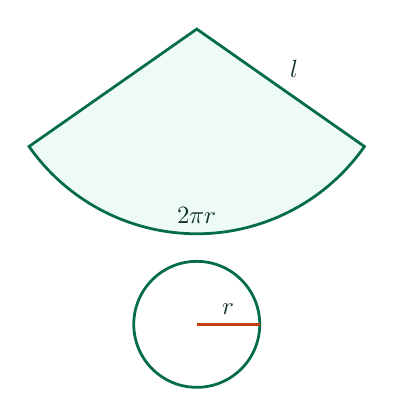
\begin{tikzpicture}
\fill[color={rgb,255:red,134;green,224;blue,189}, opacity=0.15] (0,0) -- (-35:2.6) arc[start angle=-35, end angle=-145, radius=2.6] -- cycle;
\draw[color={rgb,255:red,4;green,107;blue,77}, line width=1pt] (0,0) -- (-35:2.6) arc[start angle=-35, end angle=-145, radius=2.6] -- cycle;
\draw[color={rgb,255:red,4;green,107;blue,77}, line width=1pt] (0,-3.75) circle (0.8);
\node[font=\small, text=ink, above right] at (-35:1.3) {$l$}; \node[font=\small, text=ink, above] at (0,-2.6) {$2\pi r$};
\draw[color={rgb,255:red,194;green,65;blue,12}, line width=1pt] (0,-3.75) -- (0.8,-3.75); \node[font=\small, text=ink, above] at (0.4,-3.75) {$r$};
\end{tikzpicture}
\end{document}
